
\begin{figure}[H]
\centering
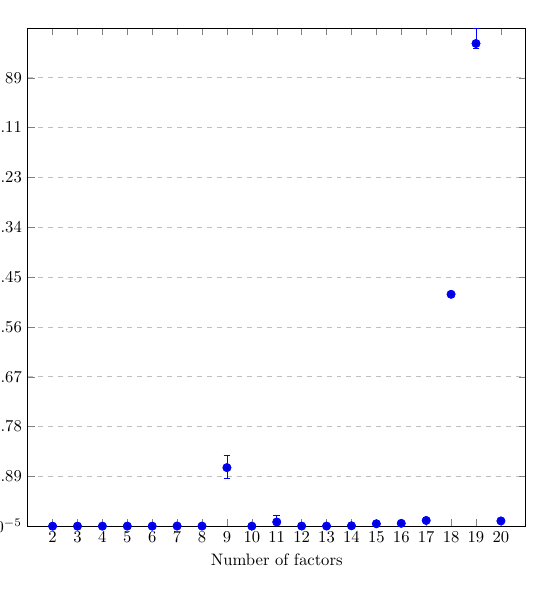
\begin{tikzpicture}[scale=0.6, trim axis left, trim axis right]
\begin{axis}[
    width=1\textwidth,
    height=1\textwidth,
    xlabel={Number of factors},
    ylabel={Time taken (s)},
    xmin=1.0, xmax=21.0,
    ymin=2.9e-05, ymax=98.893406,
    xticklabels={2, 3, 4, 5, 6, 7, 8, 9, 10, 11, 12, 13, 14, 15, 16, 17, 18, 19, 20},
    xtick={2, 3, 4, 5, 6, 7, 8, 9, 10, 11, 12, 13, 14, 15, 16, 17, 18, 19, 20},
    ytick={2.9e-05, 9.8893667, 19.7787044, 29.6680421, 39.5573798, 49.4467175, 59.3360552, 69.2253929, 79.1147306, 89.0040683},
    ymajorgrids=true,
    grid style=dashed,
]

\addplot+[
    blue,
    very thick,
    forget plot,
    only marks
    ]
    plot[
    very thick,
    error bars/.cd,
    y dir=plus,
    y explicit
    ]
    table[x=x,y=y,y error expr=\thisrow{y-max}] {
    x    y    y-max
    11	0.824594566667	1.30167143333
10	0.001	0.000348
13	0.0170693666667	0.0137016333333
12	0.0220408333333	0.0545951666667
15	0.4723911	0.0775179
14	0.0725643666667	0.0291836333333
17	1.129656	0.072157
16	0.5572707	0.0713823
19	95.8168486	3.0765574
18	46.0281998	0.2376692
20	1.0329738	0.0022332
3	0.00074864	0.00050336
2	5.128e-05	5.072e-05
5	0.01006358	0.00355642
4	0.0052101	0.1023149
7	0.02629214	0.01988286
6	0.00328196	0.00392404
9	11.6176265676	2.35868543243
8	0.01342538	0.00330362

    };

\addplot+[
    blue,
    very thick,
    forget plot,
    only marks
    ]
    plot[
    very thick,
    error bars/.cd,
    y dir=plus,
    y explicit
    ]
    table[x=x,y=y,y error expr=\thisrow{y-min}] {
    x    y    y-min
    11	0.824594566667	-0.158837566667
10	0.001	-0.000137
13	0.0170693666667	-0.00279536666667
12	0.0220408333333	-0.00490583333333
15	0.4723911	-0.0239331
14	0.0725643666667	-0.0107663666667
17	1.129656	-0.060081
16	0.5572707	-0.0202287
19	95.8168486	-0.9048276
18	46.0281998	-0.2817548
20	1.0329738	-0.0028608
3	0.00074864	-0.00021164
2	5.128e-05	-2.228e-05
5	0.01006358	-0.00171358
4	0.0052101	-0.0025821
7	0.02629214	-0.00601214
6	0.00328196	-0.00089996
9	11.6176265676	-2.05319556757
8	0.01342538	-0.00217938

    };

\end{axis}
\end{tikzpicture}
\vspace{-0.3cm}
\caption{FermatsFactorization small primes }\label{fig:FermatsFactorizationsmallprimesfactors}
\end{figure}
